%!TeX spellcheck = en-US

%\chapter{Open-set and Closed-Set Classification for WGI}
\chapter{Open-set WGI Algorithms}

\label{chap:openset}

%----------------------------------------------------------------------------------------

% Define some commands to keep the formatting separated from the content
\newcommand{\keyword}[1]{\textbf{#1}}
\newcommand{\tabhead}[1]{\textbf{#1}}
\newcommand{\code}[1]{\texttt{#1}}
\newcommand{\file}[1]{\texttt{\bfseries#1}}
\newcommand{\option}[1]{\texttt{\itshape#1}}

%----------------------------------------------------------------------------------------

\section{Introduction}\label{chap:openset:sec:intro}

WGI is a task that can be approached either as a closed-set or an open-set classification problem. The former case assumes that there is a well-defined genre palette that covers all possible genres that can be found in our domain. In addition, for each such genre there are representative instances of web-pages to be used as training data. These assumptions are far from realistic in most WGI applications. As already explained in previous chapters, it is not feasible to define a complete genre palette for the Web since there is no consensus over genre labels and new genres are emerging or existing genres evolve through time. On the other hand, it is possible to determine certain web genres where there is general agreement about their characteristics (e.g., blogs, e-shops). For such web genres it is relatively easy to find representative training data. 

Open-set classification is, therefore, a more realistic option to model the WGI task. In this setup, a genre palette covering very specific web genres is given and all other genres are considered as \textit{noise} (i.e., instances of noise should not be assigned to any of the known genres). An effective open-set WGI approach can suit any type of relevant application since it provides the ability to recognize the known web genres without being confused by the presence of noise. It should be underlined that it is expected for noise to outnumber the training instances of the known genres. Web is chaotic and of huge scale and known genres only cover a small part of it.

Open-set classifiers have to deal with an important difficulty: the \textit{Open Space Risk} (OSR). This corresponds to the instance space that lies away from the instances of known genres and can be occupied by samples of an unknown genre. An open-set classifier should be able to set the boundaries of known genres so that to avoid the risk of including an area where an unknown genre is found. This is especially challenging when the dimensionality of the representation is high. This is exactly the case with most of the popular text representation schemes that are composed of hundreds or thousands of features (e.g., character n-grams, word n-grams). It is therefore necessary to perform some kind of feature selection or to use low-dimensional feature space (e.g., word/document embeddings) when using open-set classification algorithms in WGI. 

In this chapter, three open-set WGI methods are described in detail. The first method is based on one-class classification where only positive examples are considered for each known genre. This does not mean that it is not possible to find negative examples. However, the negative class is too huge and heterogeneous that is quite challenging to extract representative negative samples. The second approach considers training samples for all available known genres and attempts to reduce the effect of high dimensionality of representation by performing repetitive subspacing. The main idea is to build an ensemble of classifiers, each one using a subset of the initial features. The third approach is an extension of the nearest-neighbor classification algorithm and attempts to directly regularize the effect of OSR.

%Finally, all three algorithms have been developed with Noise handling and Outages tolerance in mind. Specifically, all three algorithm can be tuned to regulate their Noise filtering ability with an explicit or implicit threshold. The Noise as explained earlier can be structured or unstructured, i.e. when the noise samples are balanced or not in respect of the genre tags. Note that the noise-filtering regularization threshold is automatically defined for NNDR while training using the OSR as a measure.

The rest of this chapter, first describes the main properties of open-class classification and discuss the main existing paradigms. Then, each one of the three proposed methods for WGI tasks is analytically presented. 

\section{Open-set Classification}

An open-class classification task is a tuple $(\mathcal{C},\mathcal{K},\mathcal{U})$, where $\mathcal{C}$ is a set of predefined known classes, $\mathcal{K}$ is a set of training samples for the known classes (i.e., for each $c \in \mathcal{C}$ there is a set of training samples $K_c \subset \mathcal{K}$), and $\mathcal{U}$ is a set of unknown samples to be assigned to classes. Each $u \in \mathcal{U}$ may belong to either one $c \in \mathcal{C}$ or none of them. Furthermore, the subset of $\mathcal{U}$ not belonging to any of the known classes is called noise $\mathcal{N}$.  

\subsection{Noise in Open-set Recognition}
\label{chap:openset:sec:Noise_definition}

The previous definition of open-set classification task only considers two kinds of classes, known and unknown. A more detailed analysis is provided in \parencite{geng2018recent}:

\begin{itemize}
    \item \textit{Known-known classes} are the classes for which positive samples are available. This is directly comparable to $\mathcal{C}$.
    \item \textit{Known-unknown classes} consist of negative samples that can be merged into one big artificial class, like background classes \parencite{dhamija2018reducing}.
    \item \textit{Unknown-known classes} are classes that can be described using some kind of side-information (e.g., a semantic description). However, there is lack of positive training examples for these classes. The recognition of such classes can be performed by \tetit{zero-shot learning} \parencite{palatucci2009zero}.
    \item \textit{Unknown-unknown classes} are classes without any positive training examples and without any side-information. This directly corresponds to $\mathcal{N}$. 
\end{itemize}

In this thesis we distinguish noise into unstructured and structured forms:

\begin{itemize}
    \item \textit{Unstructured Noise} corresponds to the case there is not a distinction between the unknown classes. In other words, all unknown classes are merged into a single super-class. This is very realistic in WGI applications where it is quite unclear how to define the genre of a large number of web-pages.
    \item \textit{Structured Noise} is composed of distinct unknown classes, that is we consider that each $n \in \mathcal{N}$ belongs to a class $c \notin \mathcal{C}$. Certainly, this information is not given to the open-set classifier but it is only used to estimate its performance. This is also realistic in certain WGI applications where we are interested about the recognition of specific genres and it is also known that several other genres exist.
\end{itemize}

\subsection{The Open-Space Risk}
\label{chap:openset:sec:open_space_risk}

One possibility to build classifiers that can leave some (test) instances unclassified is to introduce a reject option to closed-set classification algorithms. First, a regular closed-set classifier is trained using $\mathcal{K}$. Then, a reject criterion is determined, usually associated with the confidence of the predictions, and each test instance that does not satisfy this criterion is not classified to any of the classes in $\mathcal{C}$ \parencite{onan2018ensemble}. For example, the reject criterion could relate to the difference of probabilities assigned to the two most likely classes in $\mathcal{C}$. If this difference is large, then it is an indication that the instance in question really belongs to the most likely class (i.e., the confidence of prediction is high). If, on the other hand, the difference is small (i.e., the confidence of the prediction is low), then this means that the instance most probably does not belong to these classes. 

One big problem of this approach is that it provides strong predictions for the entire instance space. Actually, closed-set classifiers segment the instance space so that instances belonging to the known classes to be well separated. However, this also means that if an unknown class lies in the space that is far away from the known classes, it cannot be easily distinguished anymore. Figure \ref{chap:openset:fig:closed_set_classification}(a) depicts the case where a closed-set classifier is trained to recognize two known classes. Note that the decision boundary affects the entire instance space. There is also an unknown class that lies away from the known classes, almost equally away from both of them, and also near the decision boundary. This scenario can be handled by a rejection option since all members of the unknown class will be equally likely to belong to either of the known classes and, therefore, can be rejected. Figure \ref{chap:openset:fig:open_set_classification}(b) shows a similar case with two known classes and one unknown class. However, this time the unknown class lies deep in the space that seems to belong to one of the known classes. The member of unknown class are still far away from both known classes but now the rejection option will not work since it seems that one of the known classes is far more likely than the other. 

\begin{figure}[t]
	\begin{center}
    	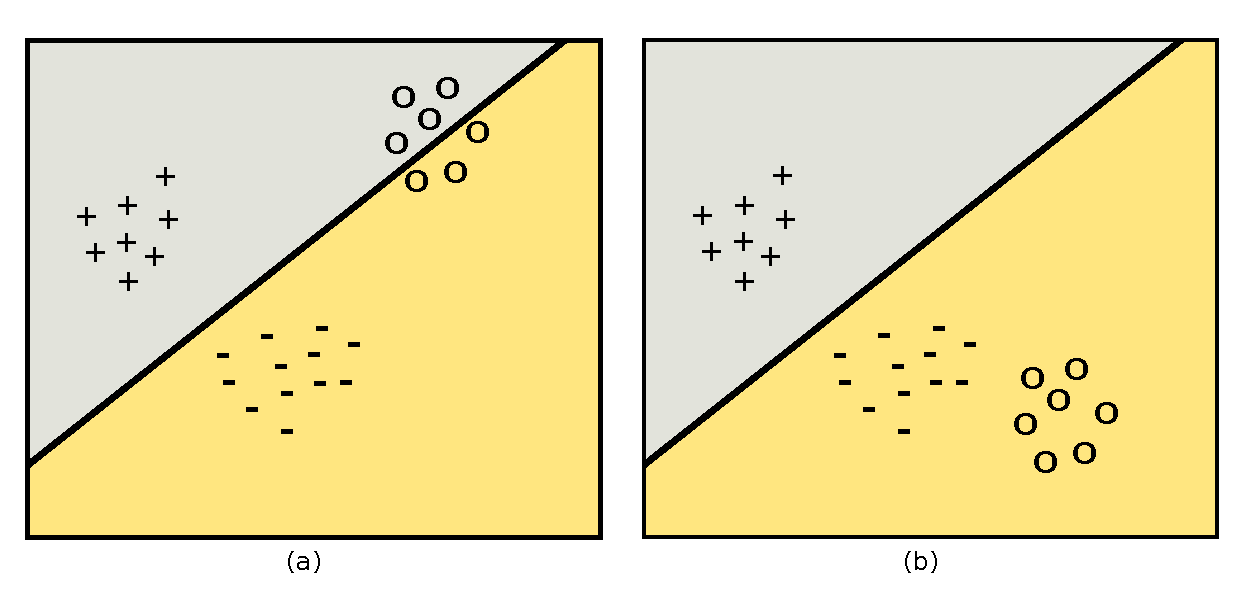
\includegraphics[scale=0.70]{Figures/closed-set_classification_schema.eps}
		\caption{An example of closed-set classification with a reject option. Known classes '+' and '-' are separated by a decision boundary. In (a) an unknown class 'o' lies away from both known classes and near the decision boundary. In (b) the unknown class lies deep in the part of one of the known classes.}
		\label{chap:openset:fig:closed_set_classification}
	\end{center}
\end{figure}


\begin{figure}[t]
	\begin{center}
    	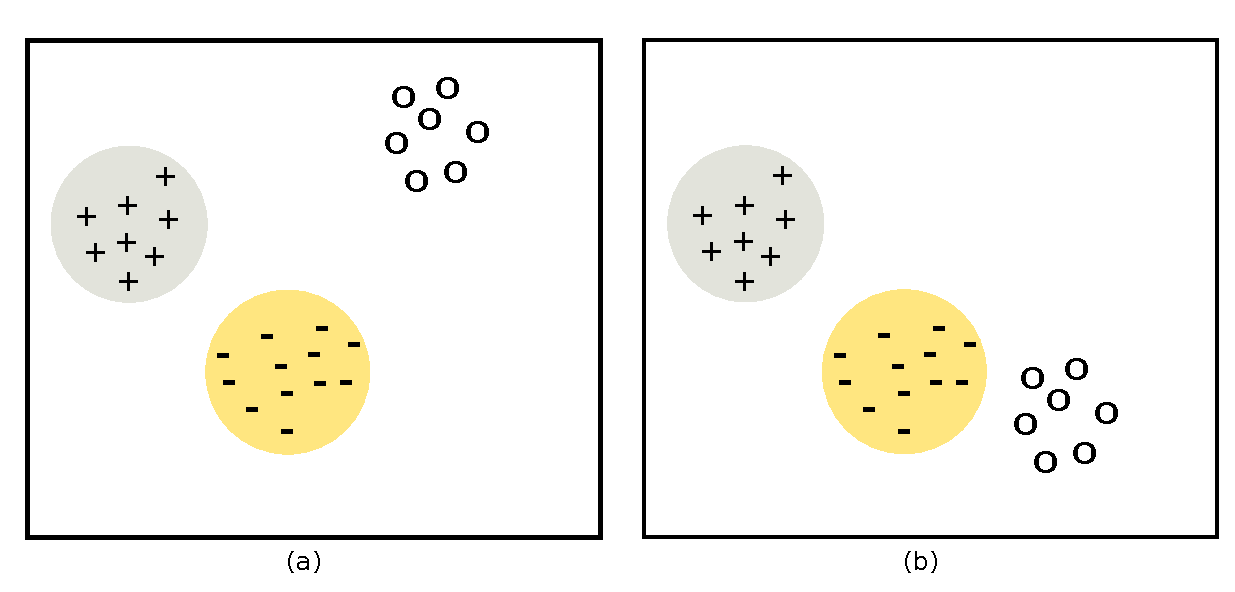
\includegraphics[scale=0.70]{Figures/open-set_classification_schema.eps}
		\caption{An example of open-set classification. Decision boundaries for known classes '+' and '-' include all positive results. In (a) an unknown class 'o' lies away from both known classes. In (b) the unknown class lies near one of the known classes.}
		\label{chap:openset:fig:open_set_classification}
	\end{center}
\end{figure}

A pure open-set classifier attempts to determine the space that surely belongs to the positive examples of each known class. An example is demonstrated in Figure \ref{chap:openset:fig:open_set_classification} where, similar to the previous case, there are two known classes and one unknown class. However, this time the relative position of the space occupied by the unknown class with respect to the position of the known classes is not that crucial anymore. In both Figure \ref{chap:openset:fig:open_set_classification}(a) and \ref{chap:openset:fig:open_set_classification}(b) the decision boundaries of known classes avoid to include samples of the unknown class.

Note that the most important issue about an open-set classifier seems to be the appropriate definition of the known class boundaries. If the classifier is too conservative, then the space allocated to the known class will be too small and it is possible to exclude some of its members. On the other hand, if the classifier is optimistic, then the area allocated to the known class will be large including neighboring areas of the known class training instances increasing the risk of including samples of unknown classes. This is demonstrated in Figure \ref{chap:openset:fig:open_space_risk_schema}. The more optimistic an open-set classifier is the more likely to suffer by the open space risk.

\begin{figure}[t]
	\begin{center}
    	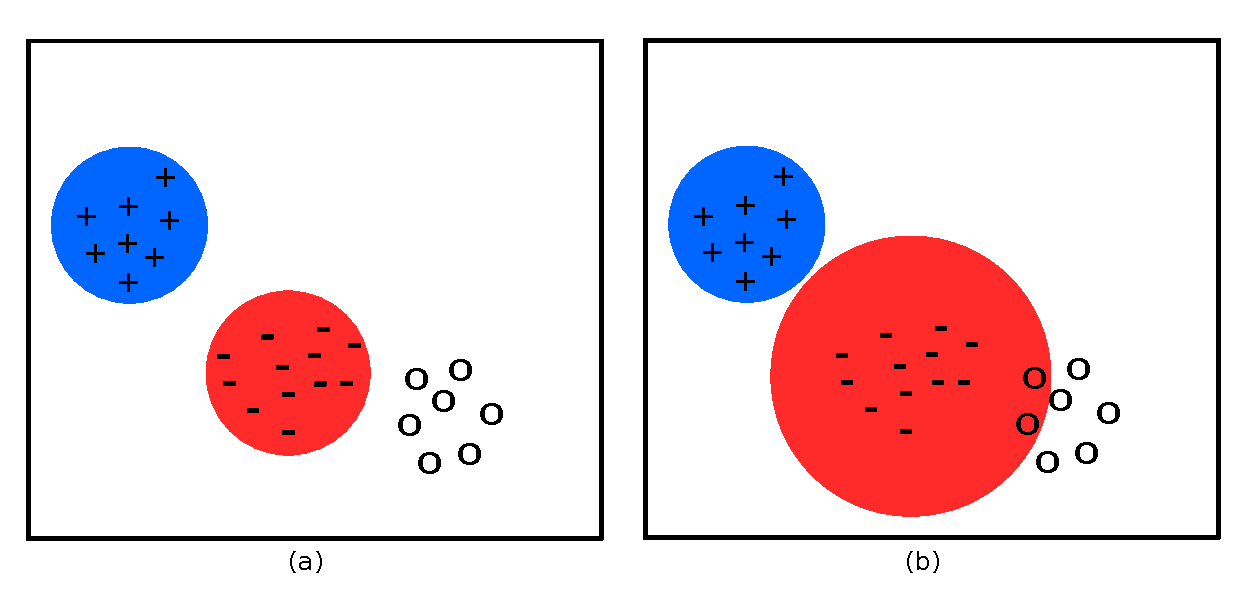
\includegraphics[scale=0.70]{Figures/open_space_risk_schema.eps}
		\caption{Open-set classification paradigm with different \textit{Open Space Risk}. Similarity case of figure \ref{chap:openset:fig:open_set_classification}. In (a) a conservative open-set algorithm is used and avoids the open space risk. In (b) an optimistic open-set algorithm is used that is more sensitive to the open space risk.}
		\label{chap:openset:fig:open_space_risk_schema}
	\end{center}
\end{figure}


Let $f_y$ be a recognition function for a known class $y$, $f_y(x)=1$ corresponds to the case $x$ is assigned to class $y$ while $f_y(x)=0$ means that $x$ is not recognized to belong to $y$. Then, the open space risk is formally defined as follows \parencite{scheirer2013toward}:

\begin{equation}\label{chap:eval_methods:eq:the_original_open_space_risk}
	R_{o}(f_y) = \frac{\int_{o} f_y(x) dx}{\int_{S_{o}}  f(x_y) dx}
\end{equation}

\noindent
where $O$ corresponds to the positively labeled open space and $S_O$ is the overall positively labeled space including the space of training samples of the known class. The larger the open space risk, the more optimistic the classifier, and the larger area is assigned to the known class.  

An alternative way to define open space is provided in  \parencite{fei2016breaking}. Let $S_O$ be a large sphere of radius $r_O$ including all positive instances of a known class and the positively labeled open space and $B_{r_y}$ be a sphere of radius $r_y$ that ideally includes all positive training examples of known class $y$. Both $S_O$ and $B_{r_y}$ have the same center $cen_y$, the center of positive training instances of class $y$. Then the open space $O$ is defined as follows:

\begin{equation}\label{chap:eval_methods:eq:openspace_spherical_constrained}
	O = S_{o} - B_{r_{y}}(cen_{y})
\end{equation}

Given this formulation, where the open space is considered as a bounded spherical area, the main issue in open-set recognition is to appropriately define radius $r_O$ for each known class.

A more formal definition of open-set classification directly involves the open space risk. Let $R_{O}$ be the open space risk and $R_{\epsilon}$ the empirical risk (i.e., the loss function in the training set). Then the objective of open-set classification is to find a function $f$ which minimizes the following \textit{open-set risk}: 

\begin{equation}
\label{eq:open_space_risk}
\argminA_{f} \{R_{O}(f ) + \lambda R_{\epsilon}(f (\mathcal{K}))\}
\end{equation}

\noindent where $f (x) > 0$ implies correct recognition and $\lambda$ is a regularization constant. Thus, open-set risk balances the empirical risk and the open space risk \parencite{geng2018recent}. 

\section{Paradigms in Open-set Classification}
\label{chap:openset:sec:Open_Set_Classification_Paradigms}

In the relevant literature, a variety of approaches to open-set recognition can be found. A thorough recent review is provided in \parencite{geng2018recent}. In general, the following main paradigms are usually followed:

\begin{itemize}
    \item One-class classification methods
    \item Modification of traditional ML methods
    \item Deep learning methods
    \item Generative models
\end{itemize}

One way to approach open-set classification is to apply \textit{One-Class classification} (OCC) methods. An OCC method is based on only positive samples of a given class. It is assumed that negative samples are either difficult to obtain or the negative class is so heterogeneous that it not easy to sample it. There are several approaches towards the solution of this problem. A compact survey on OCC is provided in \parencite{khan2010survey}. 

The \textit{Rocchio's algorithm} is the simplest one-class classification algorithm where it has been used for information retrieval tasks because of its simplicity and consistency \parencite{joachims1997probabilistic}. The learning process is just the summation of all the sample vectors of a given class, i.e the \textit{prototype vector}. Then, an arbitrary vector is classified as positive or negative using the angular distance from the prototype vector.

Datta (cited in \parencite{manevitz2002one}) proposed a Naive Bayes Classifier modification for OCC problems and use only positive samples in the learning process. A probability density function of a class $E$ is induced as prediction model. Classifying the a document $d$ involves calculating the probability of the document $p(d|E)$ which is equal to the product of its features $w_{n}$ probabilities $p(w|E)$, where $n$ is the number of document's feature vector. To decide weather the document is classified as positive, a threshold is required to be defined. 

Perhaps the most popular OCC approach is described in \parencite{scholkopf1999estimating}. It is actually a modification of the well-known SVM algorithm to the problem of the overlapping samples distributions, known as $\nu$-SVM \parencite{bishop2006}. The nature of $\nu$-SVM allows to use it in binary classification problems as long as to OCC problems. The parameter $\nu$ is both controlling the fraction of support vectors and the margin errors, i.e. positive samples considered as outliers. The optimization process begins with considering the origin as the only negative example. More details this approach are given in the section \ref{chap:openset:sec:OCSVM_description}.

Outlier-SVM is another SVM-based algorithm introduced in \parencite{manevitz2002one,khan2010survey}. The performance of this model was competitive but not top performer when compared with methods such as One Class Neural Networks, One Class Naive Bayes Classifier, One Class Nearest Neighbor, and Rocchio Prototype. In addition this algorithm is sensitive to the term weighting schema, i.e. \textit{Binary, TF, TF-IDF, etc.}, and vector dimensionality. 

There are, also, some OCC methods exploiting the availability of unlabeled data. \parencite{yu2005single} proposed two OCC algorithms that use positive and unlabeled data for building a classification model that describes the single class boundary. The \textit{Mapping Convergence}(MC) algorithm is incrementally labeling negative data from the unlabeled data set using the margin maximization property of SVM. The \textit{Support Vector Mapping Convergence} (SVMC) optimizes the MC algorithm for fast training. Both algorithms had been compared into real world  classification tasks, letter recognition, and diagnosis of breast cancer with higher performance than \textit{Spy Expectation Maximization} (S-EM), SVM-NN (i.e. C-SVM using unlabeled data point as negative ones) and Naive Bayes Classifier with noise samples \parencite{liu2002partially, li2003learning}.

In contrast to OCC, the majority of the approaches to open-set recognition are able to handle poth positive and negative samples of a given class. Several variations of well-known classification algorithms have been proposed so far. The \textit{1-vs-Set SVM} algorithm introduced in \parencite{scheirer2013toward} was the first attempt to regulate the open space based on formula \ref{eq:open_space_risk} using a second hyperplane parallel to the separating hyperplane. However, the space corresponding to each known class remains unbounded. This means that the open space risk still remains. Another SVM-based approach (W-SVM) consists of two models, a one-class SVM and a binary SVM using a Wibull cumulative distribution function \parencite{scheirer2014probability}. Yet another idea used in the POS-SVM method \parencite{scherreik2016open} models open space risk and empirical risk probabilistically. 

The \textit{Distance Based} algorithms can be adopted in the open-set framework by bounding the true positive samples by the outliers. Nearest Non-Outlier (NNO) algorithm is a center-based method that uses OSR regularization for keeping the outliers bounded. There are several center based algorithms one of them is the RFSE algorithm developed for this thesis and described in \ref{chap:openset:sec:RFSE_Description}. 

%The Nearest Neighbor algorithm which is also distance based has been adopted to the open-set framework named \textit{Nearest Neighbor Distance Ration (NNDR}). However, this algorithm it is a multi-class classification algorithm and there is no need for an adaption for this as in the above class identification cases.

%The NNDR is using he distance ration in order to regulate both the outlier bound and the OSR. Details for the NNDR are described in section \ref{chap:openset:sec:NNDR_Description} and particularly a special version of it for the WGI task developed for this thesis. It should be noted that due to its decision process where two candidate samples are selected in each step this algorithm is sensitive to outlier, however, it seems that the dimensionality of the feature space can radically change its performance as shown in chapter \ref{chap:word_embeddings}.

%The NNDR is also designed to regulate the OSR and this is part of its learning process where it divided the training data in to segments for regulating this problem in advanced. 

Deep Neural Networks are usually developed with a \textit{SoftMax} function forcing the whole modeling setup to follow a closed-set assumption. However, there have been several efforts to modify deep learning models for open-set classification, notably using \textit{OpenMax} \parencite{bendale2016towards,cardoso2017weightless}. First, a normal SoftMax model is trained. Then, the layers of the network are modified to be able to recognize (pseudo) unknown classes. Another approach is to follow the adversarial learning setup where it is attempted to generate the unknown classes. One such method, the Generative OpenMax algorithm \parencite{ge2017generative} estimates the decision boundary between known classes and the generated unknown ones.

%The \textit{Extreme Value Theory (EVT)} and \textit{Sparse Representation based} approached is an other group of ML algorithms adopted for the open-set scenario. EVT is a statistical method where the tails of the \textit{distance distributions} can be modeled using the \textit{asymptotic theory}. Thus, the distribution of the \textit{margin distance of each sample to each class} can be approximated. Then this distribution is the boundary for discarding the outlier and the rest of the unknown space (and ultimately the the open space).

%In all the open-set algorithms discussed so far and implemented of this thesis, the goal is the discovery of the threshold implicitly or explicitly, as a rejection criterion in the classification process. Thus the threshold plays a key role. Introducing threshold inevitably the OSR is introduced. An other approach for tackling this problem is the \textit{Dirichlet Process} for the open-set scenario \parencite{geng2018recent}.

Another generative approach is based on the \textit{Dirichlet Process}, a distribution over distributions. This model is not overly depended on the training samples and can adapt to changes in data distribution. The collective decision-based OSR (CD-OSR) method applies co-clustering to model each known class \parencite{geng2018collective}. Each known class can be represented by several of the obtained clusters while some clusters are not associated with any of the known classes. In the testing phase, each instance that falls into these unassociated clusters is assigned to the unknown classes. The main advantage of this generative approach over discriminative-based ones is that it does not need any threshold definition.

\section{Open-set Classifiers for WGI}
\label{chap:openset:sec:Open_set_classifiers_for_WGI}

\subsection{One-Class SVM}\label{chap:openset:sec:OCSVM_description}

The first open-set WGI method introduced in this thesis follows the OCC paradigm. Basically, the main idea is to build a one-class SVM classifier for each class $c \in \mathcal{C}$ using only the positive instances of that class. Ideally, the members of unknonwn classes will not be recognized by any of these one-class classifiers.

One-class SVM attempts to find the contour including the positive samples of the target class. Following the logic from the traditional SVM algorithm, a one-class modification, called $\nu$-SVM, was introduced in \parencite{scholkopf1999estimating}. Let $x_1, x_2,..., x_l$ be a set of positive samples of the target class and $\phi$ a feature map. $\nu$-SVM considers the origin (in feature space $\phi$) as the only negative sample and attempts to separate the positive samples from the origin and maximize the distance of the decision hyperplance from the origin. The latter is called \textit{margin} ($\rho$). More formally, the algorithm solves the following optimization problem:

\begin{equation}\label{chap:openset:sec:eq:3}
	arg\min_{w,\rho}\left\{ \frac{1}{\nu l} \sum_{i=1}^{l}(\xi_{i}-\rho)+\frac{1}{2}\|w\|^{2}\right\}
\end{equation}

\nointend subject to:

\begin{equation}
    (w \cdot \phi(x)) \geq \rho - \xi_i, \xi_i \geq 0
\end{equation}

\noindent where $\xi$ corresponds to slack variables allowing the model to handle outliers and $\nu$ a hyper-parameter in $(0,1)$. Similar to the traditional SVM, the solution involves the construction of a \textit{dual problem} where a Lagrange multiplier ($\alpha_i$) is associated with every constraint of the primary problem. Thus, the following optimization problem is solved:

\begin{equation}\label{chap:openset:sec:eq:12}
	arg\min_{\alpha}\frac{1}{2}\sum_{i,j}a_{i}a_{j}k(x_{i},x_{j})
\end{equation}

\nointent subject to:

\begin{equation}\label{chap:openset:sec:eq:4}
	0\leqslant a_{i}\leqslant \frac{1}{\nu l} %,\qquad i=1,...,l
\end{equation}

\begin{equation}\label{chap:openset:sec:eq:5}
%	\nu\leqslant\sum_{i=1}^{l}a_{i}, 
	\qquad \sum_{i=1}^{l}a_{i}=1
\end{equation}

\nointend where $k(x,y)$ is a kernel function. Non-zero $\alpha_i$ are the support vectors and only them contribute to the decision function:

\begin{equation}
    f(x) = sgn(\sum_i \alpha_i k(x_i,x) - \rho)
\end{equation}

Note that the offset $\rho$ can be derived by any support vector whose $\alpha_i$ is not at the upper or lower bound. The hyper-parameter $\nu$ has the following properties:

\begin{itemize}
	\item $\nu$ is an upper bound on the fraction of outliers.
	\item $\nu$ is a lower bound on the fraction of support vectors.
	\item $\nu$ values cannot exceed 1.
\end{itemize}

This hyper-parameter determines the smoothness of the algorithm. For small values of $\nu$, errors get penalized severely and only a few outliers are permitted. This also increases the open space risk. On the other hand, large values of $\nu$ correspond to very conservative models where a large part of  positive examples are outliers. For example in \parencite{scholkopf1999estimating} is showed that in their experiments when using $\nu=0.05$, 1.4\% of the training set has been classified as outliers while using $\nu=0.5$, 47.4\% is classified as outliers and 51.2\% is kept as support vectors.

In WGI we usually have multi-class classification problems. For each known class, a separate OCSVM model is extracted. Then, in the application phase, for each unknown sample, each OCSVM model decides whether the sample belongs to its class. In addition to a crisp decision, we also take into account the distance of the sample from the hyperplane as an indication of the confidence of this prediction. Finally, the unknown sample is assigned to the class with maximal confidence or left unclassified in case all OCSVM models reject it. 

This OCSVM approach to WGI was first introduced in \parencite{pritsos2013open} and it is analytically described in algorithm \ref{chap:openset:sec:alg:OCSVM_Ensemble} \footnote{The implementation of OCSVM in Python uses the \textit{scikit-learn} package.}.

\begin{algorithm}[t]
\caption{The \textit{OCSVM} algorithm.}\label{chap:openset:sec:alg:OCSVM_Ensemble}
\KwData{ $G$ a genre palette and $W_{g}$ a set of known web-pages for each $g \in G$,
		 $w$ an unknown webpage of the $W_{a}$ arbitrary webpages set,
		 $F$ the feature set,
		 $\boldsymbol\nu$ the nu hyper-parameter of OCSVM,
         }
\KwResult{ $r \in \{G,\,\emptyset\}$ }
$score[:, :]$=0, the score 2D matrix where rows are for genre's class tags and columns for each webpage under evaluation
\For{each $g \in G$}{
  $Model(g) = ocsvmTrain(W_{g},F,\boldsymbol\nu)$, train a OCSVM model in vector space $F$ with hyper-paramenter $\boldsymbol\nu$ for genre $g$\;
}
\For{each $g \in G$}{
    \For{each $w \in W_{a}$}{
        $score[g, w] = ocsvmApply(Model(g),F,w)$, the distance of the unknown page $w$ from the hyperplane\;
    }
}
\eIf{$max(score[:, :])< 0$}{
    $r \in \emptyset$, i.e. none of the known genres or "I don't know";
}
{
        $r = argmax_{g \in G}(score[:, :])$, i.e. $w$ belongs to the genre of highest score\;
    }
\end{algorithm}

\hfill

Note that the same hyper-parameter $\nu$ value is used for all known genres. This value should be determined empirically. OCSVM is affected by the \textit{curse of dimensionality} which causes the generalization error to increase with the number of irrelevant and redundant features \parentcite{Erfani:2016}. The following open-set classification method attempts to avoid this problem.

\subsection{Random Feature Subspacing Ensemble}\label{chap:openset:sec:RFSE_Description}

WGI tasks are usually associated with high dimensional data. In addition, the kind of features involved in text representation schemes are highly redundant and irrelevant. It is therefore crucial for an open-set classification method to handle the curse of dimensionality appropriately.

A distance-based open-set classification method has been introduced in \parencite{koppel2011authorship} aiming to handle the task of \textit{Author Identification} where similar types of problems exist with respect to WGI. In the original approach, there is only one training example for each known class and a number of simple classifiers is repetitively learned based on random feature subspacing (i.e., a randomly-selected number of features is used). Each classifier uses a similarity measure to estimate the most likely class for a given new sample. The main idea is that it is more likely for the true class to be selected by the majority of the classifiers since the used subset of features will still be able to reveal the high similarity. If, on the other hand, there is no prevailing class, then the new sample is not assigned to any of the known classes. Note that in author identification we are mainly interested about stylistic similarities. The style of the author (of genre) can be captured by many different features so a subset of them will also contain enough stylistic information (redundant features). Since WGI is also a style-based text categorization task, this idea should also work for it.

In this thesis, we adopt this method for open-set WGI tasks \parencite{pritsos2013open}. In WGI there are multiple trainig samples for each known genre. To maintain simplicity of classifiers, we have used a \textit{centroid vector} for each genre. In the training phase, a centroid vector is formed for every known class by averaging all the representation vectors of the training examples of web pages belonging to the same genre.

The class centroids are all formed for a given feature type. Then, an evaluation sample is compared against every centroid and this process is repeated $I$ times. Every time a different randomly-selected feature subset is used. Then, the scores are ranked from highest to lowest and we measure the number of times the sample is top-matched with every class. The sample is assigned to the genre with maximum number of matches given that this score exceed a predefined $\sigma$ threshold. In the opposite case, the sample remains unclassified, the RFSE responds "I Don't Know". The RFSE method is analytically described in Algorithm \ref{chap:openset:sec:alg:RFS-Ensemble}. 

\begin{algorithm}[t]
\caption{The \textit{RFSE} algorithm.}\label{chap:openset:sec:alg:RFS-Ensemble}
\KwData{ $G$ a genre palette and $W_{g}$ a set of known web-pages for each $g \in G$,
		 $w$ an arbitrary web-page of the $W_{a}$ arbitrary webpages set,
		 $F$ the feature set,
		 $fs$ a fraction of feature set size,
		 $I$ a number of iterations,
		 $\boldsymbol\sigma$ the decision threshold }
\KwResult{ $r \in \{G,\,\emptyset\}$ }
\For{each $g \in G$}{
  $centroid[g] = average(W_{g},F)$, average all known web-pages $W_{g}$ of genre $g$ to build a centroid vector\;
  $score[g]=0$\;
}
\Repeat{$I$ times}{
    $f = subset(F,fs)$, Randomly choose $fs$ features from the full feature set $F$\;
    \For{each $g$ in $G$}{
        \For{each $w$ in $W_{a}$}{
    	   $sim[g, w] = similarity(w, centroid(g), f)$, estimate similarity of unknown page $w$ with $centroid(g)$ in vector space $f$\;
        }
    }
   	$maxg = argmax_{g \in G}(sim[:, :])$, find the top match genre\;
   	$score(maxg) = score(maxg) + 1$, increase the score of top match genre\;
}

\eIf{$max(score(g))/I > \boldsymbol\sigma$}{
   $r = argmax_{g \in G}(score(g))$, assign the unknown page to genre with maximum top matches\;
}
{
      $r = \emptyset$, none of the known genres or "I don't know"\;
}
\end{algorithm}

The number of iterations and the decision threshold should be derived empirically. With respect to the similarity function used by the algorithm, there are several choices. In this thesis, we examine three options. First, the \textit{cosine similarity}, a typical selection in text mining tasks since it can easily handle high-dimensional and sparse vectors. Then, the \textit{MinMax similarity}, inspired by the excellent results reported by \parencite{koppel2014determining} in another style-based text categorization task. These two similarity measures for vectors of dimensionality $n$ are defined as follows:

\begin{equation}
\label{eq:cosine}
cosine(\vec{x},\vec{y})= \frac{\displaystyle \sum_{i=1}^{n} x_i,y_i}{(\displaystyle \sum_{i=1}^{n} x_i^2)^\frac{1}{2}×(\displaystyle \sum_{i=1}^{n} y_i^2)^\frac{1}{2}}
\end{equation}

\begin{equation}
\label{eq:minmax}
minmax(\vec{x},\vec{y})=\frac{\displaystyle \sum_{i=1}^{n}(min(x_i,y_i))}{\displaystyle \sum_{i=1}^{n} (max(x_i,y_i))}	\end{equation}

Finally, we introduce an approach that combines these two similarity functions. The idea is that the most confident measure can be used in each iteration. More specifically, since cosine and MinMax may have different mean and standard deviation for the set of all evaluation samples and all iterations per sample, their values should first be normalized. Then, for each evaluation sample and each iteration we select the one with maximum normalized value. We call this \textit{Combo} similarity measure.

\subsection{Nearest Neighbors Distance Ratio}\label{chap:openset:sec:NNRD_Description}

The approaches we consider so far use the positive training instances for the available known classes and do not attempt to estimate the open space risk. However, the distribution of known classes could be used as an indication about the existence of other unknown classes. The next algorithm attempts to follow this direction.

The Nearest Neighbors Distance Ratio (NNRD) algorithm is an open-set classification algorithm introduced in \parentcite{mendesjunior2016}, which in turn, is an extension upon the \textit{Nearest Neighbors} (NN) algorithm. The main idea is that if the new sample lies close to the training samples of a known class and far away from the closest samples of other known classes, then it most likely belongs to that class. If, on the other hand, the new sample is more or less equally distanced from the closest classes, then it should not be assigned to none of them. More formally, let $d(x,y)$ be the distance between two samples $x$ and $y$. NNRD calculates the distance of a new sample $s$ to its nearest neighbor $t$ and to the closest training sample $u$ belonging to a different class with respect to $t$. Then, if the ratio: 

\begin{equation}
    \frac{d(s,t)}{d(s,u)}
\end{equation}

\nointend is higher than a predefined threshold, the new sample is classified to the class of $s$. Otherwise, it is left unclassified. An analytical description of this approach is presented in Algorithm \ref{alg:NNDR_algorithm} \footnote{The implementation of the NNRD algorithm can be found at \url{https://github.com/dpritsos/OpenNNDR}, where it is implemented in Python/Cython and can significantly accelerated using as much as possible CPUs due to its capability for concurrent calculations in C level speed. Since, NNRD is a rather slow classification method, we have seen in practice that there is up to 100 time acceleration from the capability to exploit a cloud service with 32 vCPUs (Xeon) compare to 4-core/8-threads i7 CPU.}. 

\begin{algorithm}[t]
\caption{The \textit{NNDR} algorithm}
\label{alg:NNDR_algorithm}
\KwData{ $G$ a genre palette and $W_{g}$ a set of known web-pages for each $g \in G$,
		 $w$ an arbitrary web-page of the $W_{a}$ arbitrary web-pages set,
		 $DRT$ the distance ratio threshold}
\KwResult{ $r \in \{G,\,\emptyset\}$ }

\For{each $g \in G$}{
    \For{each $x \in W_g$}{
        $D[x] = distance(x,w)$, calculate the distance between the new web-page and the known class samples\;}
    $M[g] = minimum(D[:])$, find the minimum distance per known class\;}
$nearestNeighbor = minimum(M[:])$, find the nearest neighbor\;
$nearestClass = index(nearest_neighbor, M[:]$, find the nearest class\;
$remove(M[nearestClass],M[:])$, remove nearest class\;
$secondNearest = minimum(M[:])$, find the second nearest neighbor of another class\;
\eIf{$\frac{nearestNeighbor}{secondNearest} < DRT$}{
    $r = nearestClass$, assign $w$ to the nearest class\;}
    {$r = \emptyset$, leave $w$ unclassified\;}

\end{algorithm}

The original approach uses the Euclidean distance to find the closest neighbors. In this thesis, we use the cosine distance (i.e., 1 - cosine similarity) to better suit the properties of high dimensional and sparse data usually found in WGI tasks. 

NNDR needs a way to estimate the threshold that is appropriate for a given dataset. While traditional NN approaches in the training phase are practically idle, NNDR attempts to determine an appropriate threshold. It is remarkable that, in contrast to other open-set classifiers, training of NNDR requires both known samples (belonging to classes known during training) and unknown examples (belonging to other/unknown classes) of interest. In more detail, the \textit{Distance Ratio Threshold} (DRT) used to classify new samples is adjusted by maximizing the \textit{Normalized Accuracy} (NA):

\begin{equation}
\label{eq:normalized_accuracy}
NA = \lambda A_{KS} + (1 - \lambda) A_{US}
\end{equation}

\nointend where $A_{KS}$ is the accuracy on known samples and $A_{US}$ is the accuracy on unknown samples. The parameter $\lambda$ regulates the mistakes trade-off on the known and unknown samples prediction. Since usually in training phase only samples of known classes are available, Mendes et al. proposed an approach to repeatedly split available training classes into two sets (i.e., known and "simulated" unknown) \parentcite{mendesjunior2016}. 

In this thesis we adapt the threshold estimation process to work as follows. During the training phase the known classes are split into two sets $\mathcal{C}_K$ and $\mathcal{C}_{U}$ according to a predefined ratio $p_1$. The latter is used as the simulated unknown classes. In addition, the samples $K_c$ of each class $c \in \mathcal{C}_K$ are split into two parts $K_c^F$ and $K_c^V$ according to another predefined ratio $p_2$. The former is used as the fitting set and the latter is used as the validation set of known classes. Thus, the original training set is split into two parts the fitting set (containing the $p_2$ of the positive instances of each $c \in \mathcal{C}_K$) and the validation set (including the $(1-p_2)$ of the positive instances of each $c \in \mathcal{C}_K$ and all positive instances of each $c \in \mathcal{C}_U$). 

Then, a given range of DTR values is examined. The NNDR algorithm is called for each DTR value and the fitting set to estimate the class of each member of the validation set. That way, it is possible to calculate the $A_{KS}$ and $A_{US}$ in formula \ref{eq:normalized_accuracy} and the DTR value that maximizes normalized accuracy can be estimated. This process is repeated for all possible splits of the known classes set. In particular, given that $n = |\mathcal{C}|$ is the amount of known classes the number of splits is taken by the binomial coefficient:

\begin{equation} \label{eq:splt}
    splits(n,p_1) = \frac{n!}{\floor*{p_1n}!\floor*{(1-p_1)n}!}
\end{equation}

For example, in case we have 8 known genres and a splitting ratio $p_1=0.25$, the number of possible splits is 56. Finally the DTR value that optimizes the normalized accuracy over all splits is extracted. Note that by considering a subset of known classes as noise, the NNDR algorithm attempts to directly model the open space risk. This comes with a considerable increase in training time of the algorithm. In addition, the process of estimating DRT assumes that a big enough set of known classes is available so that a subset of them to be used as (simulated) unknown. This makes the application of this algorithm difficult in cases where there only a few known classes.

\section{Conclusions}\label{chap:openset:sec:NNRD_Description}

In this Chapter, we described three open-set classification algorithms that can be used to WGI tasks. The first method (OCSVM) follows the OCC paradigm and constructs a separate model for each known class by only considering positive instances of that class. This is a general approach that can also be used in any type of open-set classification task. In addition, this approach is expected to suffer from the curse of dimensionality, a common feature of representation schemes usually adopted in WGI. Our goal is to use this general-purpose approach as baseline for other more sophisticated methods that better suit the WGI properties.

Another proposed method (RFSE) attempts to avoid to take advantage of the curse of dimensionality focusing on random subsets of features and construct an ensemble of classifiers. Given that in style-based text categorization tasks, the representation vectors are composed by large amounts of redundant and irrelevant features, it is likely that a random subset of features will still contain enough distinguishing stylistic characteristics. The consistency of indicating a certain known genre as the most likely in the majority of such feature subsets is a strong indication of class membership. This method seems very suitable for WGI tasks. 

The last proposed method (NNDR) attempts to directly model the open space risk examining the distribution of known classes and defining simulated unknown classes. This also decreases the training phase efficiency of the method. However, given that the original NN method has zero training phase requirements, the introduced cost is not unbearable in comparison to the training time cost of other alternative classifiers. The main issue with the direct modeling of open space risk is that it makes the application of NNDR in cases with limited size of the known classes set difficult or even unfeasible (e.g., when only one known class exists). As a descendant of NN, this method also inherits its well-known problems, most crucially the difficulty to handle high-dimensional representation schemes with irrelevant features. It seems that NNDR can be effective for WGI given that an appropriate feature set is provided.